Para resolver el problema vamos a implementar la iteración de la \autoref{Eqn}
pero con la aproximación a la derivada del método elegido. 
Las funciones \texttt{pasoEU} y \texttt{pasoRK} que pueden verse
en las  \autoref{FigPasoEU} u \autoref{FigPasoRK} 

\mode*

\begin{frame}[label=FramePasoEU]
  \frametitle<presentation>{Paso para Euler}
  \begin{figure}
    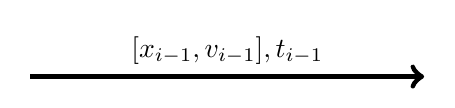
\begin{tikzpicture}[every path/.style={line width=2pt}]
      \draw[->] (0,0) -- (5, 0) node[midway, above] {$[x_{i-1}, v_{i-1}], t_{i-1}$ };
    \end{tikzpicture}
  \end{figure}
\end{frame}


\begin{figure}
  \caption{\protect\label{FigPasoRK}}
\end{figure}
